\chapter{Część teoretyczna}\label{chap:teoria}

\section{Budowa kompilatora}\label{sec:budowa_kompilatora}

Kompilator to program, który przyjmuje na wejściu reprezentację programu w
pewnym języku źródłowym i zwraca na wyjściu równoważny program w innym
języku. Językiem docelowym często bywa kod wykonywalny, bajtkod, ale może to być
też na przykład C lub JavaScript. Pod względem architektury w kompilatorach
można wyróżnić \foreign{frontend}, dokonujący przetworzenia programu wejściowego
i \foreign{backend}, generujący kod docelowy. Podział ten umożliwia utrzymywanie
wielu \foreign{frontendów} i \foreign{backendów}, na przykład w GHC dostępne są
trzy \foreign{backendy}, generujące kod maszynowy, kod w języku pośrednim LLVM
lub kod w C\cite{AOSA}. GHC może być uruchomiony w trybie interaktywnym, jako
interpreter GHCi.
%\js{Ostatnie zdanie nic nie wnosi} - GHCi pojawia się w części 4, więc chciałem o nim napomknąć

\foreign{Frontend} odpowiada za przeanalizowanie tekstu otrzymanego na wejściu
zgodnie z gramatyką języka, zbudowanie z niego drzewa składniowego i
przeprowadzenie statycznej kontroli typów. W razie błędów konieczne jest
wyświetlenie użytkownikowi wiadomości z opisem wystarczającym do jego
zrozumienia. Następnie następuje faza generowania kodu pośredniego.
Język, w którym program pisany jest przez użytkownika ma zwykle rozbudowaną składnię i jest
zaprojektowany z myślą o łatwym użytkowaniu przez ludzi. Języki pośrednie są z
kolei możliwie uproszczone pod względem składni i zaprojektowane z myślą o
dalszym przetwarzaniu przez kompilator. Kod ten przekazywany jest do
\foreign{backendu}, gdzie wykonywane są na nim optymalizacje. Możliwe jest, że
ostatnie dwie fazy powtórzą się wielokrotnie, czyli program przejdzie przez
kilka języków pośrednich i faz optymalizacji. Na koniec następuje wygenerowanie
kodu w języku docelowym\cite{Dragon}.

Glasgow Haskell Compiler ma budowę wpisującą się w ten krótki, ogólny opis. Na
schemacie \ref{fig:AOSA_compiler} można odnaleźć wymienione wcześniej fazy. W
tej pracy dokonano modyfikacji we \foreign{frontendzie}, dlatego poświęcono mu
więcej uwagi.

\begin{figure}[H]
    \centering
    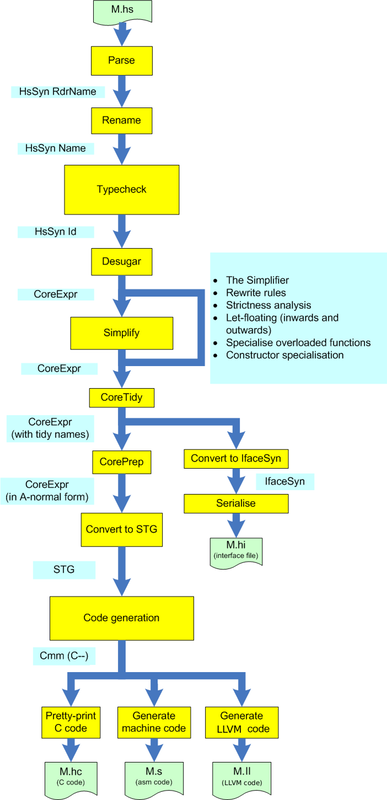
\includegraphics[width=0.7\textwidth]{images/AOSA_compiler}
    \caption[Schemat Glasgow Haskell Compiler]{Schemat Glasgow Haskell Compiler\cite{AOSA}}
    \label{fig:AOSA_compiler}
\end{figure}

\subsection{Parser}\label{sec:parser}
Parsowanie w GHC dzieli się na etapy analizy leksykalnej i składniowej. Jest to
proces tak dobrze opracowany od strony algorytmicznej, że istnieją narzędzia,
które pozwalają na generowanie gotowych lekserów i parserów z opisu gramatyki.

W czasie analizy leksykalnej plik na wejściu jest skanowany i generowany jest
z niego strumień tzw. tokenów. W GHC są to wartości typu \code{Token}
zdefiniowanego w \code{Lexer.x}. Gramatyka leksykalna jest definiowana
w postaci szeregu wyrażeń regularnych, odpowiadających kolejnym tokenom.
Lekser wyodrębnia z ciągu znaków na wejściu podciągi pasujące do wyrażeń,
czyli leksemy. Stosowana jest metoda najdłuższego dopasowania, tzn. lekser
wczytuje kolejne znaki tak długo, aż przynajmniej jedno wyrażenie akceptuje
wczytany podciąg, po czym zwraca token odpowiadający temu wyrażeniu.
Proces ten jest kontynuowany do przetworzenia całego wejścia.
%\js{Mówi Pan o leksemach, a potem w pewnym momencie pojawiają
%  się tokeny.  Może już przy pierwszej wzmiance o leksemach warto napisać, że są
%  inaczej nazywane tokenami.}
% Kierując się \cite{Dragon} postanowiłem przyjąć odrobinę różne znaczenie słów leksem i token
% "A lexeme is a sequence of characters in the source program that matches the pattern for a token and is identified by the lexical analyzer as an instance of that token."
% "A token is a pair consisting of a token name and an optional attribute value. The token name is an abstract symbol representing a kind of lexical unit..."
% Stąd leksemem nazywam ciąg znaków dopasowany do wyrażenia regularnego
% a tokenem typ danych z Lexer.x data Token = ITas | ITcase | ...

\js{(Odnośnie komentarza w kodzie źródłowym pracy: zgoda, rozumiem wytłumaczenie
  i zgadzam się z nim, ale wydaje mi się że tekst pracy nadal jest odrobinkę
  niejasny. Może spróbuje Pan to opisać tak zwyczajnie jak Pan wytłumaczył w
  komentarzu? Ponadto pierwsze zdanie akapitu mówi o generowaniu tokenów, ale
  zgodnie z tym co zrozumiałem to chyba właśnie będą ciągi leksemów?}

W GHC lekser jest generowany z wykorzystaniem narzędzia Alex. Definicja
gramatyki leksykalnej zawarta jest w pliku \code{Lexer.x}. W przykładzie
\ref{lst:alex_example} pokazane są fragmenty tego pliku. Na początku widoczne są
makra, za którymi stoją wyrażenia regularne. Na końcu fragmentu pokazane jest
kilka reguł z tymi makrami po lewej stronie i wyrażeniami, które mają zostać
zwrócone po dopasowaniu do danego wyrażenia regularnego. Znajdujące się tam
\code{idtoken}, \code{varid} itd. to zwykłe funkcje w Haskellu, zdefiniowane w
innym miejscu, które zwracają tokeny\cite{DocsAlex}.

\begin{lstlisting}[float,label={lst:alex_example},
                   caption={Wycinki z pliku \code{Lexer.x} składające się na reguły opisujące co jest wyodrębniane jako zmienna i konstruktor.}]
$unilarge  = \x01 -- Trick Alex into handling Unicode. See alexGetByte.
$asclarge  = [A-Z]
$large     = [$asclarge $unilarge]

$unismall  = \x02 -- Trick Alex into handling Unicode. See alexGetByte.
$ascsmall  = [a-z]
$small     = [$ascsmall $unismall \_]

$ascdigit  = 0-9
$unidigit  = \x03 -- Trick Alex into handling Unicode. See alexGetByte.
$digit     = [$ascdigit $unidigit]

$digit     = [$ascdigit $unidigit]
$suffix    = \x07 -- Trick Alex into handling Unicode. See alexGetByte.
$idchar    = [$small $large $digit $suffix \']

@varid     = $small $idchar*          -- variable identifiers
@conid     = $large $idchar*          -- constructor identifiers

@qual = (@conid \.)+
@qvarid = @qual @varid
@qconid = @qual @conid

haskell :-
<0,option_prags> {
  @qvarid                       { idtoken qvarid }
  @qconid                       { idtoken qconid }
  @varid                        { varid }
  @conid                        { idtoken conid }
}
\end{lstlisting}

W czasie analizy składniowej strumień tokenów zamieniany jest w bardziej złożoną
strukturę, drzewo składniowe. W GHC parser, tak jak lekser, został wygenerowany
automatycznie przy użyciu narzędzia Happy. Definicja gramatyki w formacie akceptowanym
przez Happy znajduje się w pliku \code{Parser.y}. Jest podana w notacji Backusa-Naura
wzbogaconej, podobnie jak w Alex, o fragmenty kodu w Haskellu wywoływane w celu
stworzenia struktury danych reprezentującej to drzewo\cite{DocsHappy}. Przykład
\ref{lst:happy_example} pokazuje wybrane produkcje z tego pliku, wykorzystujące
przy tym token \code{ITvarid} zwracany przez funkcję \code{varid} z przykładu
\ref{lst:alex_example}.
{
\begin{lstlisting}[float,label={lst:happy_example},
                   caption={Wycinki z pliku \code{Parser.y} z produkcjami odpowiadającymi za zmienne typów, wykorzystujące tokeny, których dotyczył przykład \ref{lst:alex_example}.}]
%token
 VARID          { L _ (ITvarid    _) }          -- identifiers
 CONID          { L _ (ITconid    _) }

tyvar   :: { Located RdrName }
tyvar   : tyvarid               { $1 }

tyvarid :: { Located RdrName }
        : VARID            { sL1 $1 $! mkUnqual tvName (getVARID $1) }
        | special_id       { sL1 $1 $! mkUnqual tvName (unLoc $1) }
        | 'unsafe'         { sL1 $1 $! mkUnqual tvName (fsLit "unsafe") }
        | 'safe'           { sL1 $1 $! mkUnqual tvName (fsLit "safe") }
        | 'interruptible'  { sL1 $1 $! mkUnqual tvName (fsLit "interruptible") }
\end{lstlisting}

\subsection{Renamer}\label{sec:renamer}

W Haskellu, jak w wielu innych językach, może istnieć kilka funkcji, zmiennych,
typów danych, klas, itd. o tej samej nazwie, na przykład w różnych plikach albo
przez występowanie w lokalnym zakresie w wyrażeniu \code{let} lub
\code{where}. Z tego powodu później ten sam identyfikator może odnosić się do
różnych rzeczy, w zależności od tego, gdzie występuje i co w tym miejscu jest
widoczne w zakresie. Kompilator, w części zwanej renamerem, decyduje, do
której definicji odnosi się każde wystąpienie jakiejś nazwy.

Każda osobna definicja otrzymuje na tym etapie unikalną, wewnętrzną
nazwę. Następnie nazwy w programie są zamieniane na odniesienia do jednej z tych
zmiennych. Utrzymywany jest w tym celu słownik nazw znajdujących się w danej
chwili w zakresie. Jeżeli w danym miejscu nie da się na podstawie zawartości
słownika jednoznacznie określić, do czego odnosi się pewne wystąpienie nazwy, to
wywoływany jest błąd jak w przykładzie \ref{lst:renamer_ambiguous}. W algorytmie
brane jest przy tym pod uwagę, czy nazwa jest kwalifikowana i w jaki sposób
importowany jest inny moduł, co może usunąć wieloznaczność. Możliwe jest również
zjawisko zwane \foreign{shadowingiem}, polegające na zastąpieniu w zakresie nazw
innych konstrukcji przez lokalną definicję, które widać na fragmencie
\ref{lst:renamer_shadowing}. Wreszcie, jeżeli w danym miejscu w zakresie nie
będzie nic o danej nazwie, to renamer zakończy działanie z błędem, jak w
przykładzie \ref{lst:renamer_missing}.

\begin{lstlisting}[float,label={lst:renamer_ambiguous},
                   caption={Przykład działania renamera - niejednoznaczne odwołanie.}]
import Data.Maybe (isJust)

isJust :: Maybe a -> Bool
isJust Nothing = False
isJust _ = True

main :: IO ()
main = print $ isJust (Just 0)

{- Wywołuje błąd:
renamer.hs:8:16:
    Ambiguous occurrence ‘isJust’
    It could refer to either ‘Main.isJust’, defined at renamer.hs:4:1
                          or ‘Data.Maybe.isJust’,
                             imported from ‘Data.Maybe’ at renamer.hs:1:20-25
-}
\end{lstlisting}

\begin{lstlisting}[float,label={lst:renamer_shadowing},
                   caption={Przykład działania renamera - shadowing.}]
foo = 10

main :: IO ()
main = let foo = 20 in print foo

-- Po uruchomieniu wypisze 20
\end{lstlisting}

\begin{lstlisting}[float,label={lst:renamer_missing},
                   caption={Przykład działania renamera - nieodnalezienie w zakresie.}]
main :: IO ()
main = print bar

-- Wywołuje błąd:
-- renamer3.hs:2:14: Not in scope: ‘bar’
\end{lstlisting}

Na tym etapie kompilacji wykonywane jest również wiele pobocznych zadań, na
przykład wyświetlenie ostrzeżeń, gdy pewna zmienna zostanie zdefiniowana, lecz
nie będzie później użyta w wyrażeniu przy kompilacji z flagą
\code{-fwarn-unused-matches}. Ta czynność jest jednym z usprawnień w tej pracy.

\subsection{Type checker}\label{sec:type_checker}

Warto w tym miejscu wspomnieć o podstawowych pojęciach związanych z systemami
typów. Częścią definicji języka jest jego gramatyka, która określa, jakie ciągi
znaków można uznać za program w tym języku. W skład gramatyki wchodzą wyrażenia,
które w wielu językach można podzielić na termy i typy.

Termy pozwalają wyrażać obliczenia dzięki zdefiniowanej dla nich semantyce.
Jednym z rodzajów semantyki jest semantyka operacyjna, w której wykonywanie
obliczeń modeluje się za pomocą maszyny stanowej. Term jest lub, w bardziej
złożonych semantykach, zawiera się w stanie maszyny. Ponadto istnieje relacja
przejścia, określającej stany do jakich przechodzi maszyna w wyniku obliczeń.
Semantykę operacyjną określa się przez przez podanie reguł ewaluacji, z których
wynika ta relacja.

Wykonywanie programu może zatrzymać się w stanie uważanym za końcowy. Term
w postaci do jakiej zostaje znormalizowany w stanie końcowym nazywamy wartością.

Obliczenia mogą też się nigdy nie zatrzymać lub utknąć w stanie, który nie jest
końcowy, lecz dla którego relacja przejścia nie określa dalszych kroków.
Termy, dla których taki jest rezultat, nazywamy niepoprawnymi lub
bezsensownymi\cite{TAPL} jak na przykładzie \ref{lst:types_nonsense}.

\begin{lstlisting}[float,label={lst:types_nonsense},
                   caption={Przykład bezsensownego wyrażenia w programie, z błędem GHC, który wywołuje.}]
module Nonsense where

nonsense = 10 + "a"

{- Błąd kompilacji w GHC:
[1 of 1] Compiling Nonsense         ( nonsense.hs, nonsense.o )

nonsense.hs:3:15:
    No instance for (Num [Char]) arising from a use of ‘+’
    In the expression: 10 + "a"
    In an equation for ‘nonsense’: nonsense = 10 + "a"
-}
\end{lstlisting}

Typy są przyporządkowywane termom w relacji typowania wynikającej z pewnych
reguł typowania. Zbiór tych reguł składa się na system typów. System typów służy do
wykrywania bezsensownych termów bez ich ewaluowania, często już na etapie kompilacji.
System typów jest konkluzywny lub bezpieczny,
\js{Dowiedziałem się ostatnio, że soundness jest w Polsce tłumaczone jako
  poprawność, natomiast completness tłumaczy się jako pełność (preferencja
  Warszawy) albo zupełność (preferencja Wrocławia).}
jeżeli każdy term, który ma w nim przyporządkowany typ, jest sensowny. Z kolei
jest zupełny, jeżeli każdy sensowny term jest w nim otypowany. Systemy typów w
popularnych językach są przeważnie konkluzywne, lecz nie zupełne. Rozszerzenia
systemu typów dążą do zmniejszenia liczby poprawnych programów, które są w
systemie typów niedopuszczalne, co można określić jako zwiększenie jego
ekspresywności. Rozszerzenia mogą doprowadzić do tego, że problem sprawdzenia,
czy dany program jest poprawnie otypowany, stanie się nierozstrzygalny. Nie
będzie wtedy możliwe stworzenie odpowiedniego algorytmu i zagwarantowanie, że
proces kompilacji się zakończy. Może to być niedopuszczalne ze względu na
oczekiwania użytkowników - programistów\cite{TAPL}.

\begin{lstlisting}[float,label={lst:types_diverge},
                   caption={Przykład programu, dla którego statyczne sprawdzanie typów w GHC się nie zakończy.}]
{-# LANGUAGE TypeFamilies, UndecidableInstances #-}

module Diverge where

type family Diverge a where
   Diverge a = Diverge a

evil :: Diverge Int
evil = 0
\end{lstlisting}

Polimorfizm to możliwość posiadania przez term więcej niż jednego przypisanego
mu typu. Może on wtedy występować w miejscach, gdzie oczekiwany jest term jednego
z tych typów.

W polimorfizmie parametrycznym uzyskuje się to przez wprowadzenie
do typu zmiennych, za które mogą być podstawiane inne typy. Termy otypowane w ten
sposób muszą mieć sens niezależnie od tego, jakie typy zostaną przyporządkowane
zmiennym, choć np. w Haskellu istnieje możliwość wprowadzenia ograniczeń na zmienne.
Polimorfizm parametryczny odpowiada kwantyfikacji ogólnej z logiki. Typy takie
mogą mieć składnię pozwalającą na zapisanie jawnego kwantyfikatora, wiążącego
zmienne w typie, zamiast pozostawiania tych zmiennych jako niezwiązanych.
W przykładzie \ref{lst:poly_parametric} funkcja \code{twice} jest polimorficzna,
w jednym miejscu zmienna \code{a} służy za \code{Bool}, a w drugim za \code{String}.
Funkcja \code{twice'} pokazuje wspomnianą jawną kwantyfikację, lecz poza tym jest
równoważna poprzedniej funkcji. W języku Java polimorfizm parametryczny
dostępny jest pod postacią typów generycznych.

\begin{lstlisting}[float,label={lst:poly_parametric},
                   caption={Przykład użycia polimorfizmu parametrycznego w Haskellu.}]
{-# LANGUAGE ExplicitForAll #-}

twice :: (a -> a) -> a -> a
twice f = f . f

twice' :: forall a . (a -> a) -> a -> a
twice' f = f . f

main :: IO ()
main = do
    print $ twice not True         -- True
    print $ twice ('-':) "Hello"   -- "--Hello"
\end{lstlisting}

W polimorfizmie ad hoc term może mieć przypisane różne typy dzięki temu,
iż ma wiele definicji. W zależności od typu wykorzystywana jest inna z nich.
W Haskellu ten polimorfizm jest dostępny w postaci klas typów\cite{TAPL}.
W przykładzie \ref{lst:poly_adhoc} funkcja \code{foo} występuje raz jako
funkcja typu \code{Bool -> Int} i raz jako \code{String -> Int}. W każdym
przypadku ma inną definicję, sensowną dla wybranego wtedy typu. W Javie
polimorfizm ten występuje pod postacią przeładowania metod, jak w przykładzie
\ref{lst:poly_adhoc_java} z metodą \code{bar}.

\begin{lstlisting}[float,label={lst:poly_adhoc},
                   caption={Przykład użycia polimorfizmu ad hoc w Haskellu.}]
class C a where
    foo :: a -> Int

instance C Bool where
    foo True = 1
    foo _    = 0

instance C [a] where
    foo = length

main :: IO ()
main = do
    print $ foo True      -- 1
    print $ foo "Hello"   -- 5
\end{lstlisting}

\begin{lstlisting}[float,language=Java,label={lst:poly_adhoc_java},
                   caption={Przykład użycia polimorfizmu ad hoc w Javie.}]
public class Parametric {
    public static void main(String... args) {
        bar(10);       // bar int 10
        bar("str");    // bar String str
    }

    static void bar(int arg) {
        System.out.println("bar int " + arg);
    }

    static void bar(String arg) {
        System.out.println("bar String " + arg);
    }
}
\end{lstlisting}

W kompilatorze sprawdzenie, czy program jest poprawnie otypowany, zachodzi w części
zwanej type checkerem. Jednym z zadań type checkera jest wyświetlenie w razie błędu takich
komunikatów, by pozwolić użytkownikowi zrozumieć problem i go naprawić.
Z tego powodu aż do tego etapu kompilacji zachowywane są takie informacje
jak lokalizacja w pliku wejściowym i identyfikatory wybrane przez użytkownika.

\section{Rozszerzenia Glasgow Haskell Compiler}\label{sec:rozszerzenia_ghc}

Przez rozszerzenia GHC rozumiane są zaimplementowane w nim funkcje, które nie są
częścią specyfikacji języka przedstawioną w Haskell 2010 Language
Report. Zliczenie linii w rezultacie wywołania \code{ghc --supported-extensions}
pozwala stwierdzić, że jest ich obecnie około stu. Rozszerzenia są opcjonalne i
domyślnie wyłączone. Uaktywnia się je dyrektywą języka umieszczoną na początku
pliku modułu lub przez podanie odpowiednich flag wśród argumentów wywołania
kompilatora. Wszystkie zmiany wykonane w tej pracy wiążą się z pewnymi
rozszerzeniami, dlatego warto je omówić.

\subsectionex{Rodziny typów}{Rozszerzenie \code{TypeFamilies}}\label{sec:rodziny_typow}

Rodziny typów to funkcje operujące na typach w trakcie kompilacji.
Stworzenie rodziny typów wymaga podania deklaracji rodziny z liczbą i rodzajami
parametrów oraz pewnej liczby definicji lub równań. W przypadku rodzin związanych
z klasą, deklaracja znajduje się w deklaracji klasy i musi wykorzystywać parametry
klasy. Przykładem takiej rodziny jest \code{Box} z klasy \code{T} na
fragmencie \ref{lst:typefams_assoc_standalone}. Może dodatkowo
posiadać równanie domyślne, o takim samym znaczeniu co domyślne definicje
funkcji w klasie. Równania podaje się przy definiowaniu instancji klasy. W
przypadku rodzin niezależnych od klasy, jak \code{Cont} z przykładu
\ref{lst:typefams_assoc_standalone}, deklarację tworzy się z użyciem słowa
kluczowego \code{family}, a równania tworzy się ze słowem kluczowym \code{instance}.

\begin{lstlisting}[float,label={lst:typefams_assoc_standalone},
                   caption={Przykład pozwiązanej z klasą i niezależnej rodziny typów.}]
{-# LANGUAGE TypeFamilies #-}

module TypeFamilies where

class T a where
    data Box a
    store :: Box a -> a -> Box a

instance T Int where
    data Box Int = BoxI0 | BoxI1 Int
    store BoxI0 n = BoxI1 n
    store (BoxI1 acc) n = BoxI1 $ acc + n

instance T Bool where
    data Box Bool = BoxB0 Int Int
    store (BoxB0 ts fs) True = BoxB0 (ts + 1) fs
    store (BoxB0 ts fs) _    = BoxB0 ts (fs + 1)


data family Cont a
data instance Cont Int = ContI0 | ContI1 Int
data instance Cont Bool = ContB0 Int Int

class S a where
    put :: Cont a -> a -> Cont a

instance S Int where
    put ContI0 n = ContI1 n
    put (ContI1 acc) n = ContI1 $ acc + n

instance S Bool where
    put (ContB0 ts fs) True = ContB0 (ts + 1) fs
    put (ContB0 ts fs) _    = ContB0 ts (fs + 1)
\end{lstlisting}

Rodziny typów dzielą się na rodziny synonimów typów, deklarowane ze słowem
kluczowym \code{type} i rodziny typów danych, deklarowane ze słowem
kluczowym \code{data}. Równania należące do rodzin synonimów tworzą synonimy typów,
podobne do tych z nierozszerzonego Haskella. W przykładzie \ref{lst:typefams_open_close}
\code{Equal Int Int} jest synonimem \code{Int} i oba równie dobrze mogą znaleźć
się w deklaracji typu dla \code{foo}. Analogicznie, rodziny typów danych grupują
typy danych \code{data} lub \code{newtype}. Na przykład \code{Cont Int} z przykładu
\ref{lst:typefams_assoc_standalone} to nazwa typu danych, którego wartości konstruuje się
z użyciem \code{ContI0} lub \code{ContI1}.

Rodziny synonimów mieć postać otwartą i zamkniętą. W formie
zamkniętej wszystkie równania rodziny wymienione są w miejscu jej
deklaracji. Mają tę zaletę wobec rodzin otwartych, iż poszczególne równania mogą na
siebie nachodzić i w takim wypadku stosowany jest synonim, którego równanie jest
pierwsze od góry. Przypomina to mechanizm dopasowania wzorców dostępny na poziomie
termów. W przypadku rodzin otwartych, kolejność równań nie jest
określona i mogą one być definiowane w wielu plikach, więc nachodzenie na siebie
dziedzin równań powoduje błąd. Różnicę tę widać w przykładzie
\ref{lst:typefams_open_close}\cite{GuideTypeFamilies}.

\begin{lstlisting}[float,label={lst:typefams_open_close},
                   caption={Przykład otwartej i zamkniętej funkcji na typach z nachodzącymi na siebie dziedzinami.}]
{-# LANGUAGE TypeFamilies #-}

module TypeFamilies where

type family Equal a b where
    Equal a a = a
    Equal a b = (a, b)

foo :: Equal Int Int
foo = 10

type family Open a b
type instance Open a a = a
type instance Open a b = (a, b)

{-
families-overlapping.hs:13:15:
    Conflicting family instance declarations:
      Open a a -- Defined at families-overlapping.hs:13:15
      Open a b -- Defined at families-overlapping.hs:14:15
-}
\end{lstlisting}

\subsectionex{Częściowe sygnatury typów}{Rozszerzenie \code{PartialTypeSignatures}}\label{sec:partial_sigs}

W Haskellu, podczas definiowania wyrażenia, możliwe i zwykle zgodne z dobrymi
praktykami jest dopisanie sygnatury typu. Jest to jednak opcjonalne, gdyż przy
braku sygnatury w czasie sprawdzania typów dojdzie do próby
rekonstrukcji. Istnieje jednak również inna, pośrednia opcja: podanie niepełnej
sygnatury, zawierającej tak zwane symbole wieloznaczne, zapisywane w postaci
podkreślnika.

Domyślnie obecność wieloznacznika wywoła błąd, w którego treści znajdzie się
zrekonstruowany typ, którym można uzupełnić sygnaturę, a kompilacja zostanie
przerwana. Rozszerzenie \code{PartialTypeSignatures} zmieni jednak to
zachowanie, sprawiając, iż zamiast błędu wygenerowane zostaną jedynie
ostrzeżenia i obecność wieloznacznika nie będzie przyczyną zakończenia działania
kompilatora. Dodatkowo ostrzeżenia te można ukryć uruchamiając GHC z flagą
\code{-fno-warn-partial-type-signatures}. Przykład
\ref{lst:partialsigs_infer_type} demonstruje przebieg kompilacji z tym
rozszerzeniem.

\begin{lstlisting}[float,label={lst:partialsigs_infer_type},
                   caption={Przykład użycia anonimowego symbolu wieloznacznego w sygnaturze typu.}]
foo :: _ -> Bool
foo = not

{- Wywoła błąd lub ostrzeżenie:
partial.hs:3:8:
    Found hole ‘_’ with type: Bool
    To use the inferred type, enable PartialTypeSignatures
    In the type signature for ‘foo’: _ -> Bool
-}
\end{lstlisting}

Symbol wieloznaczny może także znaleźć się wśród ograniczeń klasowych jak w
przykładzie \ref{lst:partialsigs_infer_constraints}. Wtedy w błędzie lub
ostrzeżeniu, generowanym na takich samych zasadach, co w poprzednim przypadku,
znajdą się wywnioskowane przez kompilator zero lub więcej ograniczeń. Oprócz
wieloznacznika w sygnaturze mogą znaleźć się jawnie podane ograniczenia.

\begin{lstlisting}[float,label={lst:partialsigs_infer_constraints},
                   caption={Przykład użycia anonimowego symbolu wieloznacznego w ograniczeniach typu.}]
bar :: _ => [a] -> Bool
bar (x:y:_) = x == y
bar _ = False

{- Wywoła błąd lub ostrzeżenie:
partial-constr.hs:3:8:
    Found hole ‘_’ with inferred constraints: (Eq a)
    To use the inferred type, enable PartialTypeSignatures
    In the type signature for ‘bar’: _ => [a] -> Bool
-}
\end{lstlisting}

Drugim rozszerzeniem związanym z częściowymi sygnaturami jest
\code{NamedWildCards}. Sprawia ono, iż identyfikatory zaczynające się od
podkreślnika są również traktowane jako wieloznaczniki i są traktowane w podobny
sposób do tego zaprezentowanego w \ref{lst:partialsigs_infer_type} i
\ref{lst:partialsigs_infer_constraints}. Bez niego wyłącznie same podkreślniki
są traktowane jako wieloznaczniki, a identyfikatory zaczynające się od
podkreślników jako zwyczajne zmienne typów. Opcjonalne aktywowane wieloznaczniki
określane są jako wieloznaczniki nazwane, a te opisane poprzednio jako
wieloznaczniki anonimowe.

Warte uwagi jest, iż nazwane wieloznaczniki to nie zmienne typów. Pokazuje to
przykład \ref{lst:partialsigs_named_wcs}, gdzie po aktywowaniu rozszerzenia
\code{NamedWildCards} podana sygnatura jest poprawna, z wywnioskowanym typem
\code{Bool} w miejscu \code{\underscore x}. Bez tego rozszerzenia z kolei jest
ona niepoprawna, gdyż \code{\underscore x} jest wtedy traktowana jako zwykła
zmienna, a zatem \code{foo} jest wtedy funkcją polimorficzną, która powinna mieć
sens dla każdego \code{\underscore x}, co wyraźnie nie jest prawdą dla wyrażenia
\code{not \underscore x}\cite{GuidePartialTypeSignatures}.

\begin{lstlisting}[float,label={lst:partialsigs_named_wcs},
                   caption={Demonstracja różnicy między zmienną z podkreślnikiem i nazwanym wieloznacznikiem.}]
omodule Partial where
foo :: _x -> (Bool, _x)
foo a = (True, not a)

foo :: _ -> Bool
foo = not

{- Wywoła błąd lub ostrzeżenie:
partial-named.hs:4:16:
    Couldn't match expected type ‘_x’ with actual type ‘Bool’
      ‘_x’ is a rigid type variable bound by
           the type signature for foo :: _x -> (Bool, _x)
           at partial-named.hs:3:8
    Relevant bindings include
      a :: _x (bound at partial-named.hs:4:5)
      foo :: _x -> (Bool, _x) (bound at partial-named.hs:4:1)
    In the expression: not a
    In the expression: (True, not a)
-}
{- Z rozszerzeniem NamedWildCards:
partial-named.hs:3:8:
    Found hole ‘_x’ with type: Bool
    To use the inferred type, enable PartialTypeSignatures
    In the type signature for ‘foo’: _x -> (Bool, _x)
-}
\end{lstlisting}
